
	There were five applications developed that can be separated into two groups. The first group is the \ac{Wiimote} device group, the second is the Kinect device group. The Wiimote group has three distinct applications, an interface application, a solver application, and a control application. The Kinect group has an interface application and a control application. The structure of the two common applications is the same, only being distinguished by its inner logic.
	
		\begin{figure}[htb]
	\centering
	  \subfloat[Simple representation of Yarp Device Driver main classes.] {\label{fig:deviceApp}\includegraphics[scale=0.30,page=4,angle=90]{icubSimpleNetworkDiagram-crop.pdf}}
  \hspace{5mm}
	  \subfloat[Simple representation of the Interaction Module main classes.] {\label{fig:controlApp}\includegraphics[scale=0.30,page=5,angle=90]{icubSimpleNetworkDiagram-crop.pdf}}
	  \caption{Interaction applications structure.}
	  \label{fig:interactionApps}
	\end{figure}
	
	The interface application implements the \ac{Yarp} device abstraction. This application is responsible for streaming the data from the interface device into a \ac{Yarp} port in a simple and usable format, so that other programs can take advantage from that data by connecting to the port or using it as an \ac{Yarp} device. The control application uses the \ac{Yarp} device abstraction implemented by the interface application. This application is responsible for converting the data retrieved from the interface application into values that are used to control the iCub. Figure \ref{fig:deviceApp} shows the main classes of the interface and control applications, in the case of the \ac{Wiimote} the control application is also responsible for altering the settings of the \ac{Wiimote}.
	
	As can be easily seen by the figure both applications have a device interface driver class that inherits from the RFModule and TypedReaderCallback classes. The functionality of this common class is similar in both cases. Both applications have a data receiving port that executes a function per each set of data received, and a data sending port that is maintained by a thread that writes data to that port. This system enables communication between this two modules, or other helper modules that might be implemented. An example of a helper module is the \ac{Wiimote} solver application which is used to decide based on the \ac{MP} data which is the best position for the end-effector to try and reach.
	
	The applications were developed using C++ and used the \ac{Yarp} and iCub libraries. For the development of the interface applications, two extra libraries were used to get data from the devices the wiiuse library\footnote{\url{http://sourceforge.net/projects/wiiuse/}} and the OpenNI/NITE library\footnote{\url{http://www.openni.org/}}. The wiiuse library\footnote{\url{http://sourceforge.net/projects/wiiuse/}} was used to get data and set settings of the \ac{Wiimote}. The wiiuse version used was altered by the fwiineur library\footnote{\url{http://fwiineur.blogspot.com/search/label/release}} developers so that data from the \ac{MP} could be retrieved. The OpenNI/NITE library uses the \ac{IR} projector and \ac{IR} camera from the Kinect to calculate a depth map. Using this depth map and the NITE algorithms it is possible retrieve a set of rotation matrices or points that describe the pose and position of a users body or body parts.